\documentclass[12pt]{article}


\usepackage{amssymb}
\usepackage{amsmath}
\usepackage{fullpage}
\usepackage{epsfig}
\usepackage{epstopdf}
\everymath{\displaystyle}

\newif\ifans

\ansfalse

\begin{document}

\begin{center}
\underline{\LARGE{Area As A Limit \& Sigma Notation}}
\end{center}

\noindent SUGGESTED REFERENCE MATERIAL:

\bigskip

\noindent As you work through the problems listed below, you should reference Chapter 5.4 of the recommended textbook (or the equivalent chapter in your alternative textbook/online resource) and your lecture notes.

\bigskip

\noindent EXPECTED SKILLS:

\begin{itemize}

\item Understand and know how to evaluate the summation (sigma) notation. 

\item Be able to use the summation operation's basic properties and formulas. (You do not need to memorize the ``Useful Formulas" listed below; if they are needed, they will be provided to you). 

\item Know how to denote the approximate area under a curve and over an interval as a sum, and be able to find the exact area using a limit of the approximation. 

\item Be able to find the net signed area between the graph of a function and the $x$-axis on an interval using a limit.

\end{itemize}

\noindent USEFUL FORMULAS\\

\bigskip

\begin{tabular}{p{0.3\linewidth} p{0.35\linewidth} p{0.33\linewidth}}
$\sum_{k=1}^n{k}=\frac{n(n+1)}{2}$ & $\sum_{k=1}^n{k^2}=\frac{n(n+1)(2n+1)}{6}$ & $\sum_{k=1}^n{k^3}=\left(\frac{n(n+1)}{2}\right)^2$
\end{tabular}\\

\bigskip

\noindent PRACTICE PROBLEMS:

\medskip

\noindent {\bf For problems 1-5, evaluate.}

\begin{enumerate}

\item $\sum\limits_{k=1}^{4}k^3$ 

\ifans{\fbox{100}} \fi

\item $\sum\limits_{j=2}^{6} (j^3-1)$ 

\ifans{\fbox{435}} \fi

\item $\sum_{i=-1}^3{2i}$

\ifans{\fbox{10}} \fi

\item $\sum_{k=0}^5{(-1)^k}$

\ifans{\fbox{0}} \fi

\item $\sum_{k=1}^5{\sin{\left(\frac{\pi}{2}k\right)}}$

\ifans{\fbox{1}} \fi

\end{enumerate}

\noindent {\bf For problems 6-8, use the summation formulas at the top of page 1 to evaluate the given sum.}

\begin{enumerate}
\setcounter{enumi}{5}

\item $\sum_{k=1}^{100}{(3k-5)}$

\ifans{\fbox{14,650}} \fi

\item $\sum\limits_{k=1}^{25}[ k(k-1)(k+1)]$ 

\ifans{\fbox{105,300}} \fi

\item $\sum_{k=3}^{120}{(k+7)}$\\

(CAUTION: In problem 8, the lower index is not 1; so, the summation formulas at the top of page 1 do not immediately apply!)

\ifans{\fbox{8,083}} \fi

\end{enumerate}

\noindent {\bf For problems 9-12, write the given expression in sigma notation.  Do not evaluate the sum.  (For each, there are many different ways to write the expression in sigma notation; the answer key illustrates one such way for each.))}

\begin{enumerate}
\setcounter{enumi}{8}

\item $4(1)+4(2)+4(3)+4(4)+\dots +4(20)$ 

\ifans{\fbox{$\sum_{k=1}^{20}4k$}} \fi

\item $3-6+9-12+ \dots -36$ 

\ifans{\fbox{$\sum_{k=1}^{12}3(-1)^{k+1}k$}} \fi

\item $1+3+5+7+ \dots + 21$

\ifans{\fbox{$\sum_{k=0}^{10}(2k+1)$}} \fi

\item $2+4+8+16+ \dots + 256$

\ifans{\fbox{$\sum_{k=1}^{8}2^k$}} \fi

\end{enumerate}

\noindent {\bf For problems 13-15, express the given summation in closed form.}

\begin{enumerate}
\setcounter{enumi}{12}

\item $\sum\limits_{j=1}^{n}\frac{j}{n}$ 

\ifans{\fbox{$\frac{n+1}{2}$}} \fi

\item $\sum\limits_{k=1}^{n-1} \frac{3k^3}{n}$ 

\ifans{\fbox{$\frac{3n(n-1)^2}{4}$}} \fi

\item $\sum\limits_{k=0}^{n} \left(\frac{1}{n}-\frac{k^2}{n}\right)$ \\
(CAUTION: In problem 15, the lower limit is not 1; so the summation formulas at the top of page 1 do not immediately apply!)

\ifans{\fbox{$1-\frac{(n+1)(2n+1)}{6}+\frac{1}{n}$}} \fi

\item Consider $f(x)=x^2+1$.

\begin{enumerate}

\item Estimate the area under the graph of $f(x)$ on the interval $[0,6]$ using 3 rectangles of equal width and right endpoints, as in the diagram below.  Is your estimate an overestimate or an underestimate?

\begin{center}

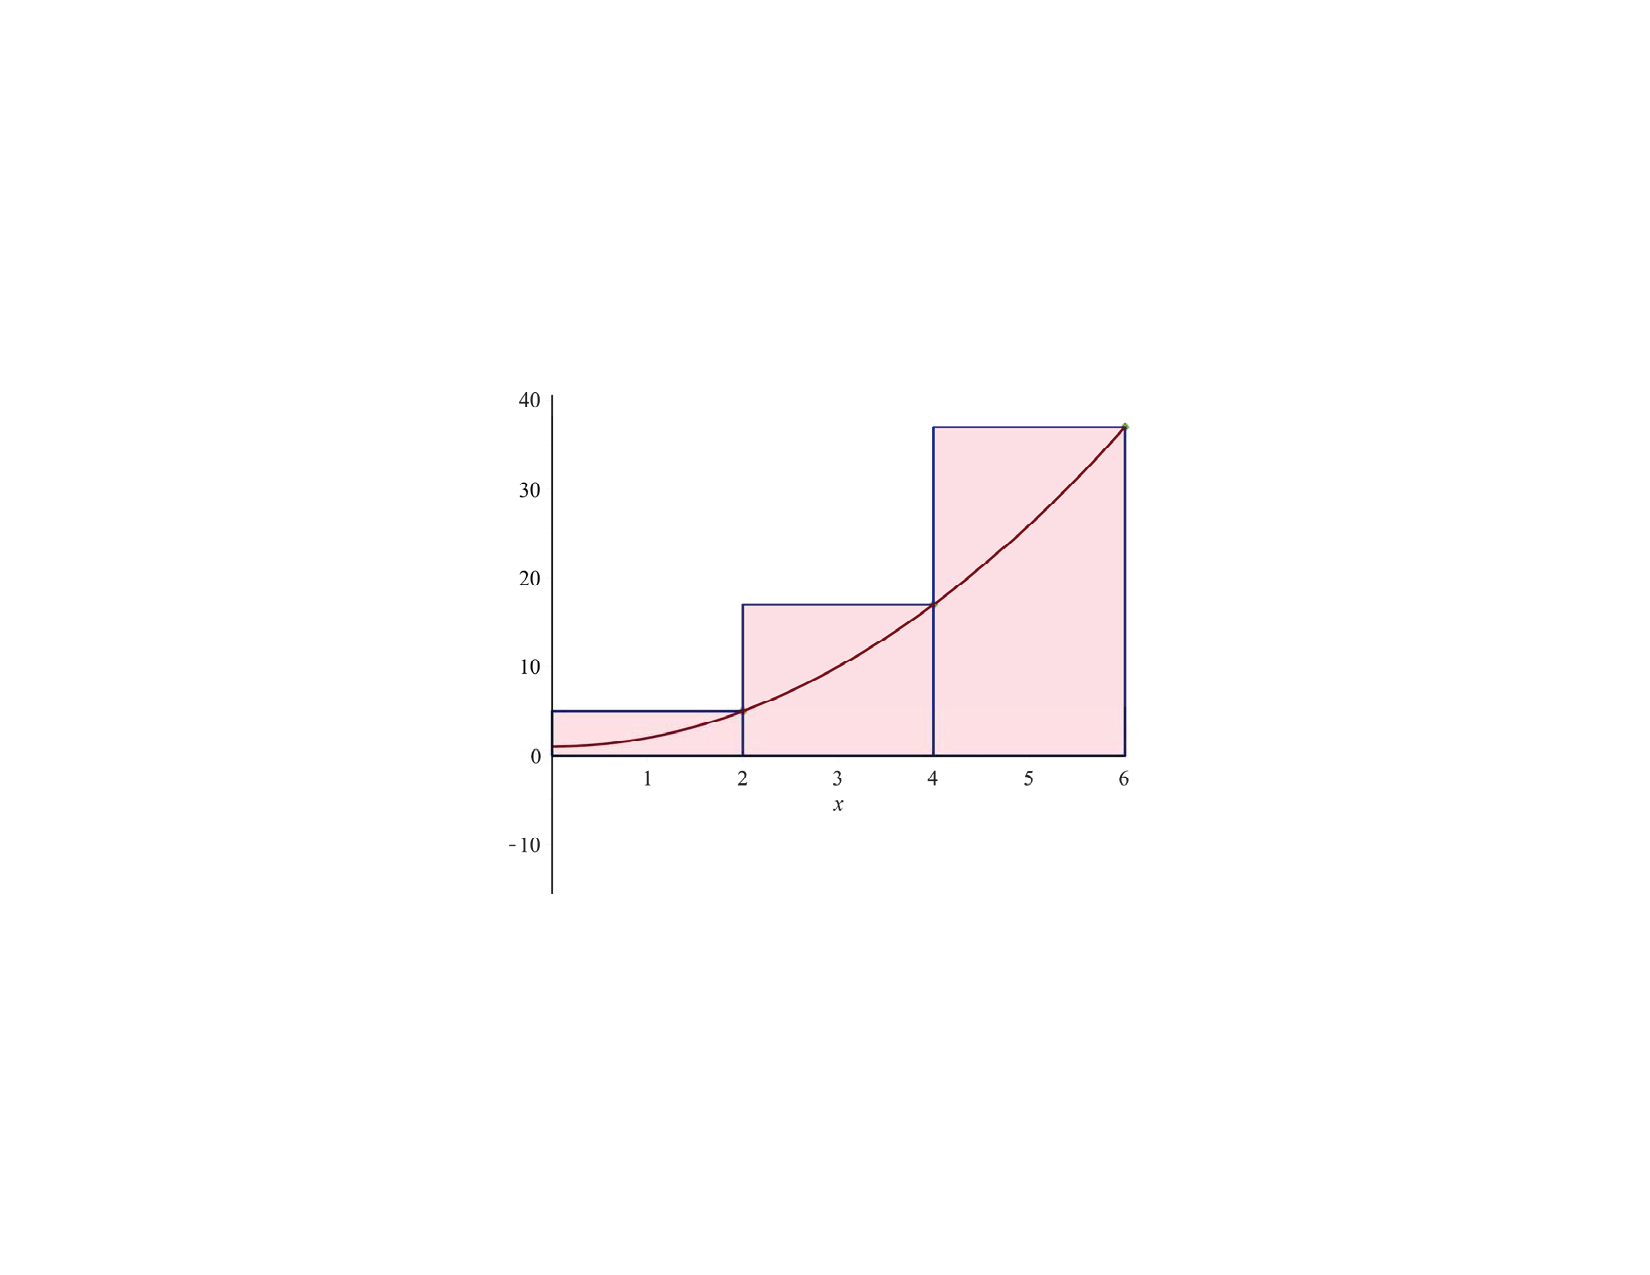
\includegraphics[scale=0.5]{x2+1right.pdf}

\end{center}

\ifans{\fbox{$A \approx 118$; It is an overestimate.}} \fi

\item Estimate the area under the graph of $f(x)$ on the interval $[0,6]$ using 3 rectangles of equal width and left endpoints, as in the diagram below.  Is your estimate an overestimate or an underestimate?

\begin{center}

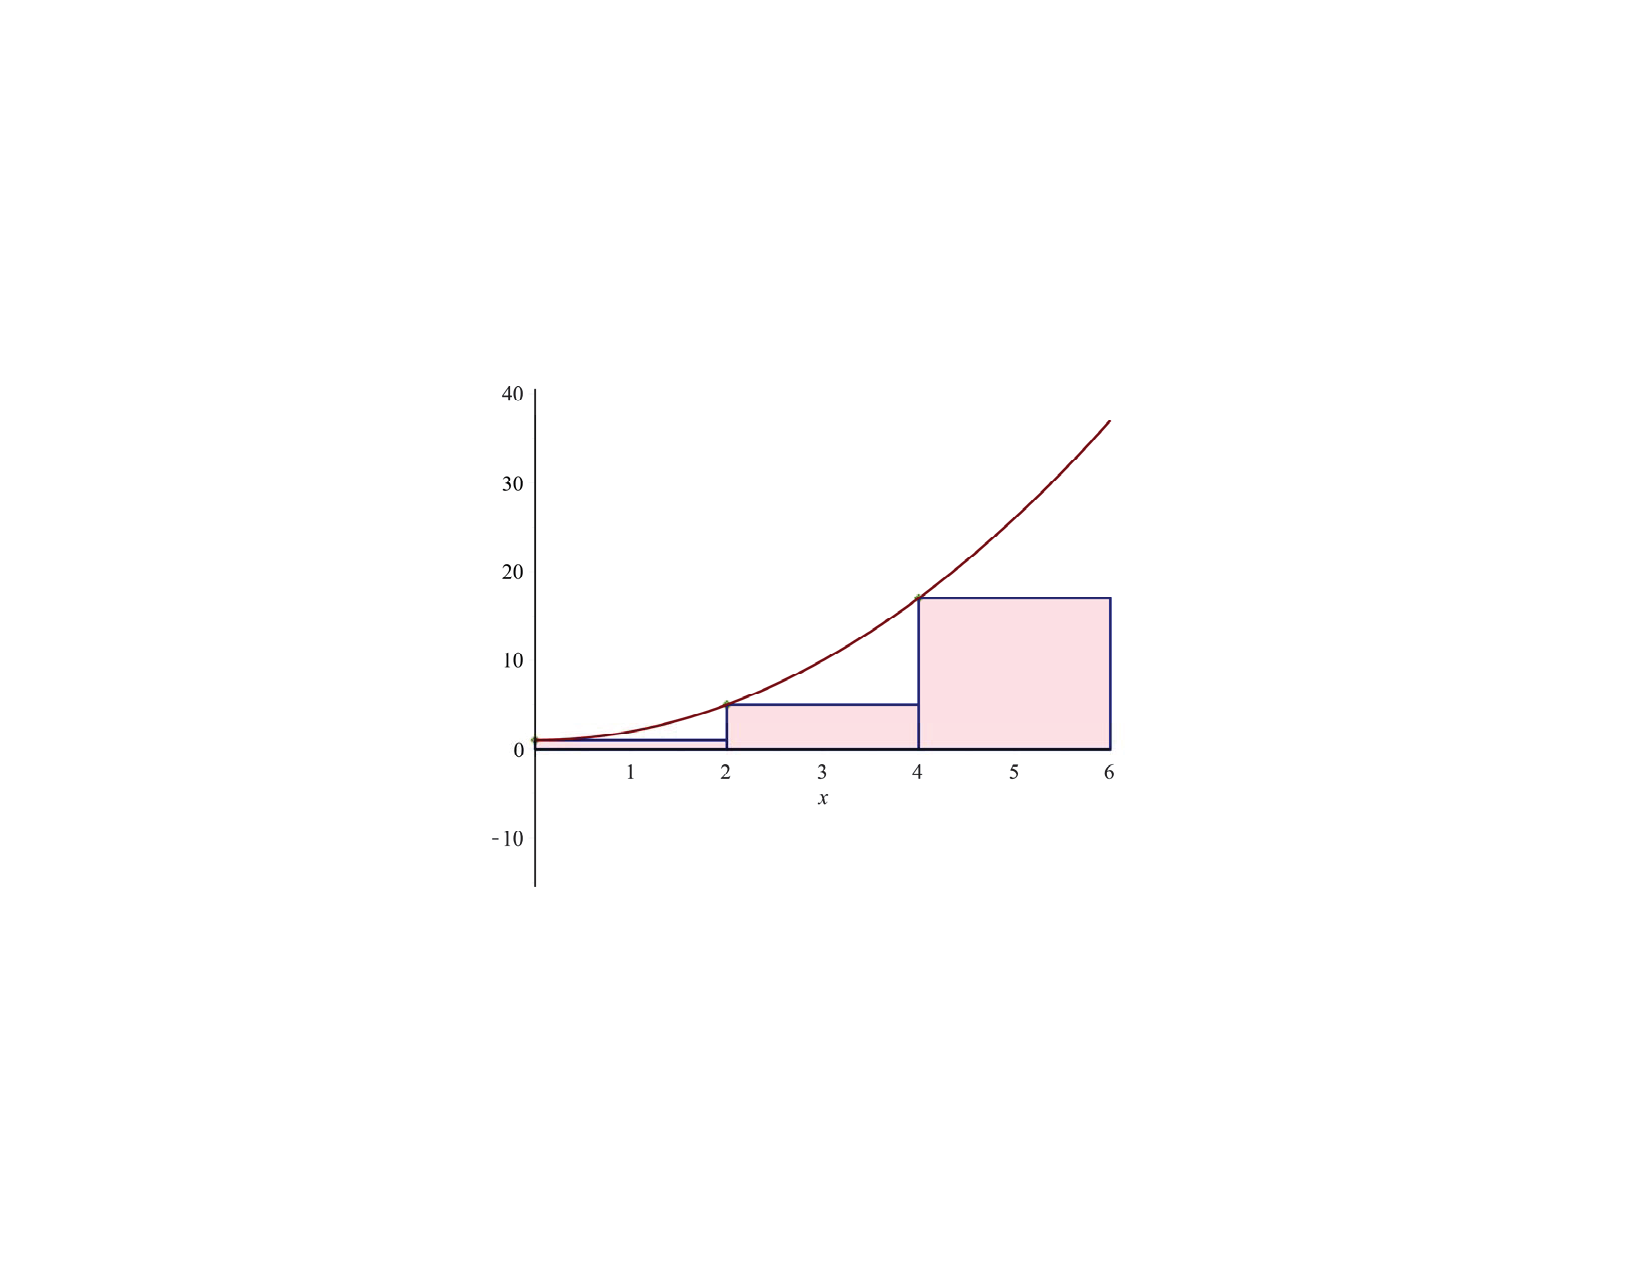
\includegraphics[scale=0.45]{x2+1left.pdf}

\end{center}

\ifans{\fbox{$A \approx 46$; It is an underestimate.}} \fi

\item Estimate the area under the graph of $f(x)$ on the interval $[0,6]$ using 3 rectangles of equal width and midpoints, as in the diagram below.  Is your estimate an overestimate or an underestimate?

\begin{center}

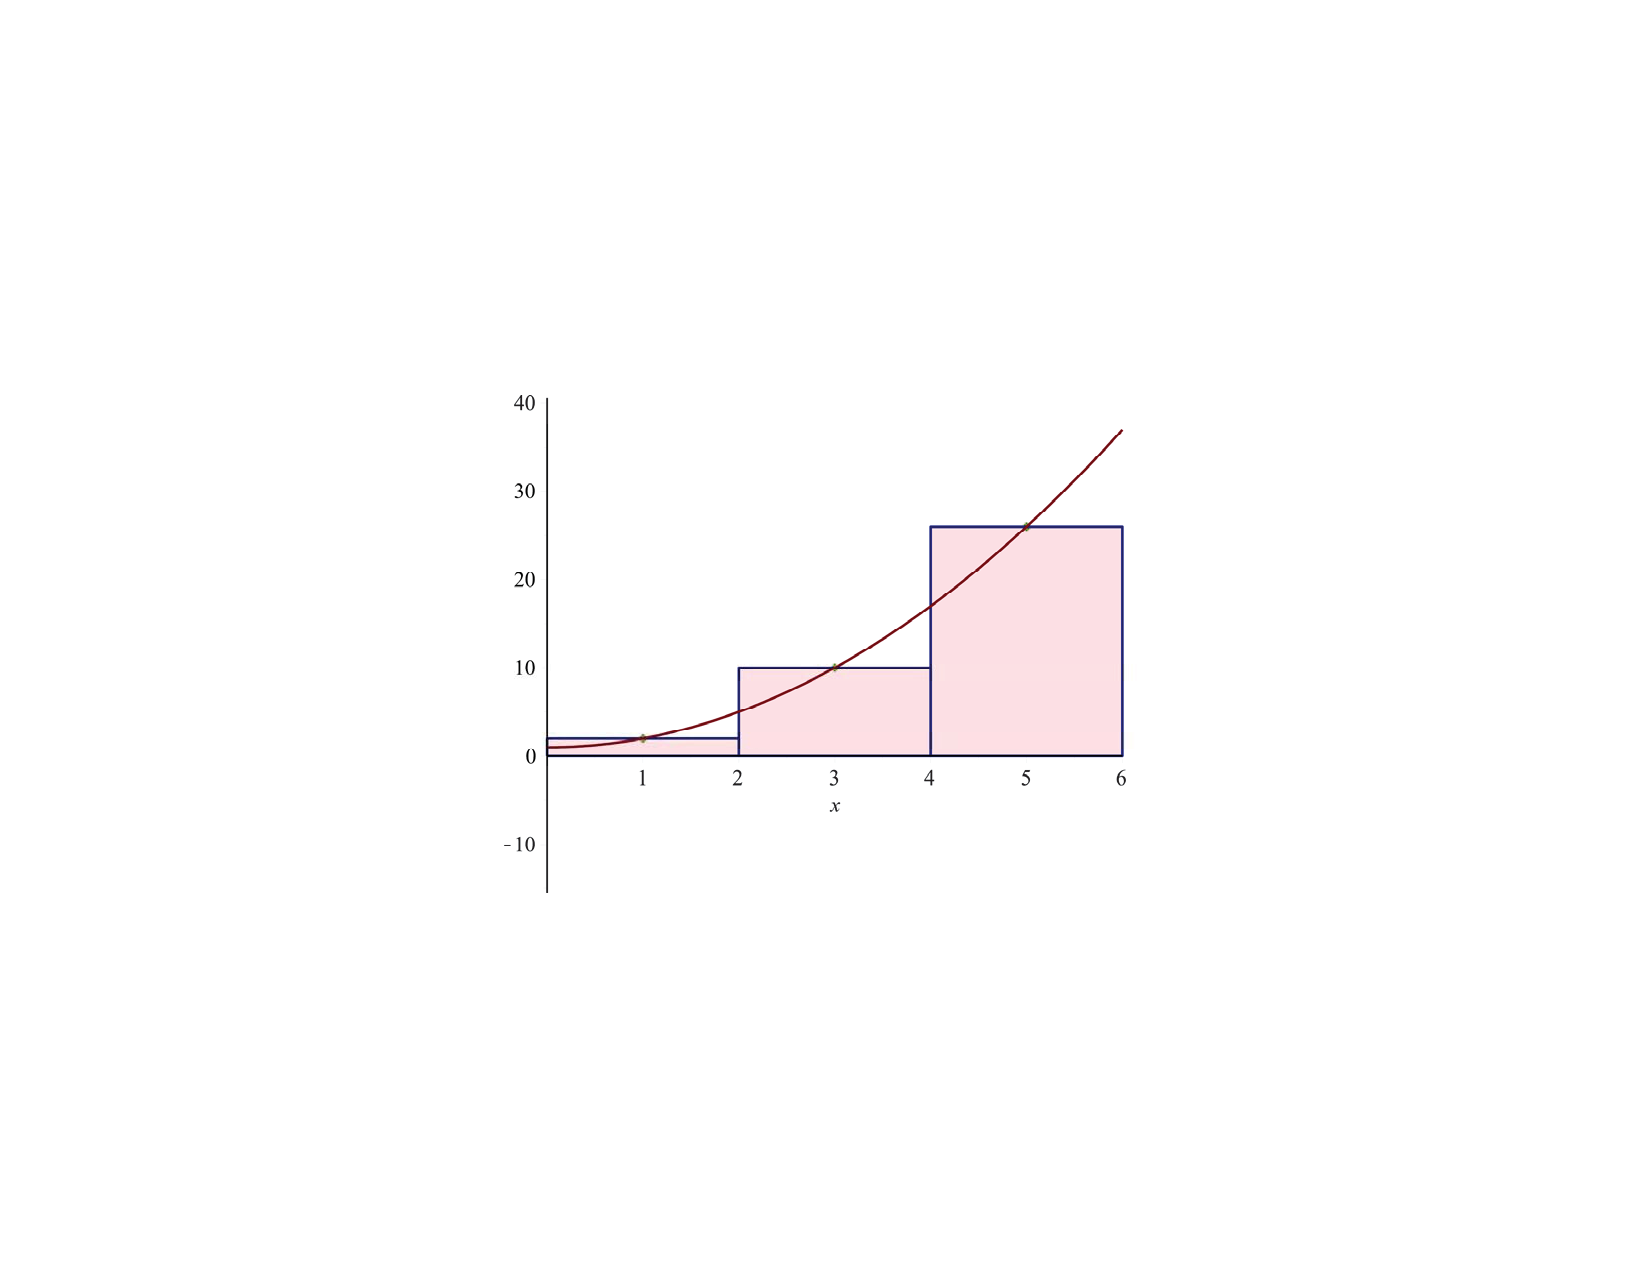
\includegraphics[scale=0.45]{x2+1mid.pdf}

\end{center}

\ifans{\fbox{\parbox{1\linewidth}{$A \approx 76$; By inspection, it is hard to judge whether this is an overestimate or an underestimate.  In fact, in a future section, you will be able to show that the exact area is 78.}}} \fi

\end{enumerate}

\newpage

\item Let $f(x)=\ln{x}$.

\begin{enumerate}

\item Sketch the graph of $f(x)$.  Label all asymptotes and intercepts with the coordinate axes.

\ifans{\fbox{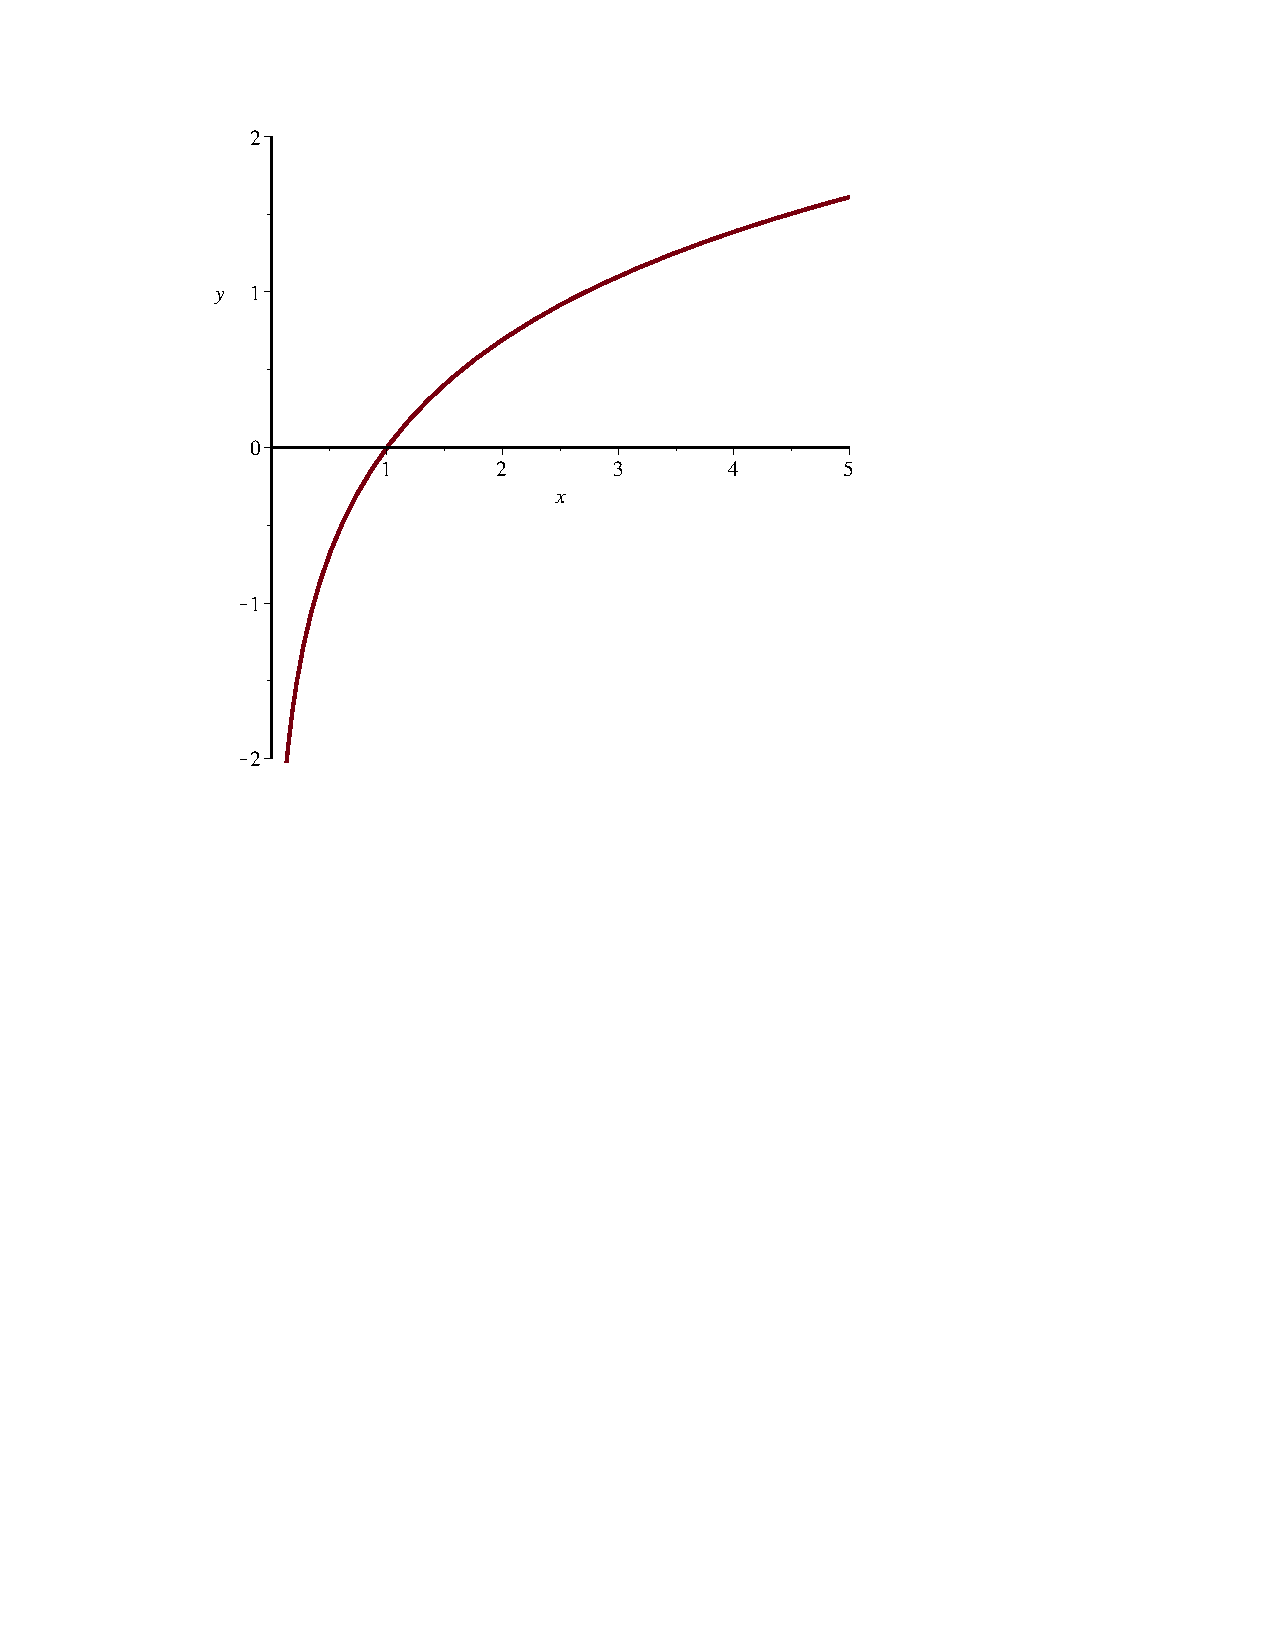
\includegraphics[scale=0.4]{log.pdf}}} \fi

\item Sketch the graph of $f(x)$ on the interval $[e,5e]$.  Divide the interval into 4 subintervals of equal width.  On each subinterval, sketch a rectangle using the function value at the {\bf right endpoint} as the height of the rectangle on that subinterval.  Estimate the area between the graph of $f(x)$ and the $x$-axis on the interval $[e,5e]$ using the 4 rectangles that you sketched.  Is your estimate an overestimate or an underestimate?

\ifans{\fbox{\parbox{0.65\linewidth}{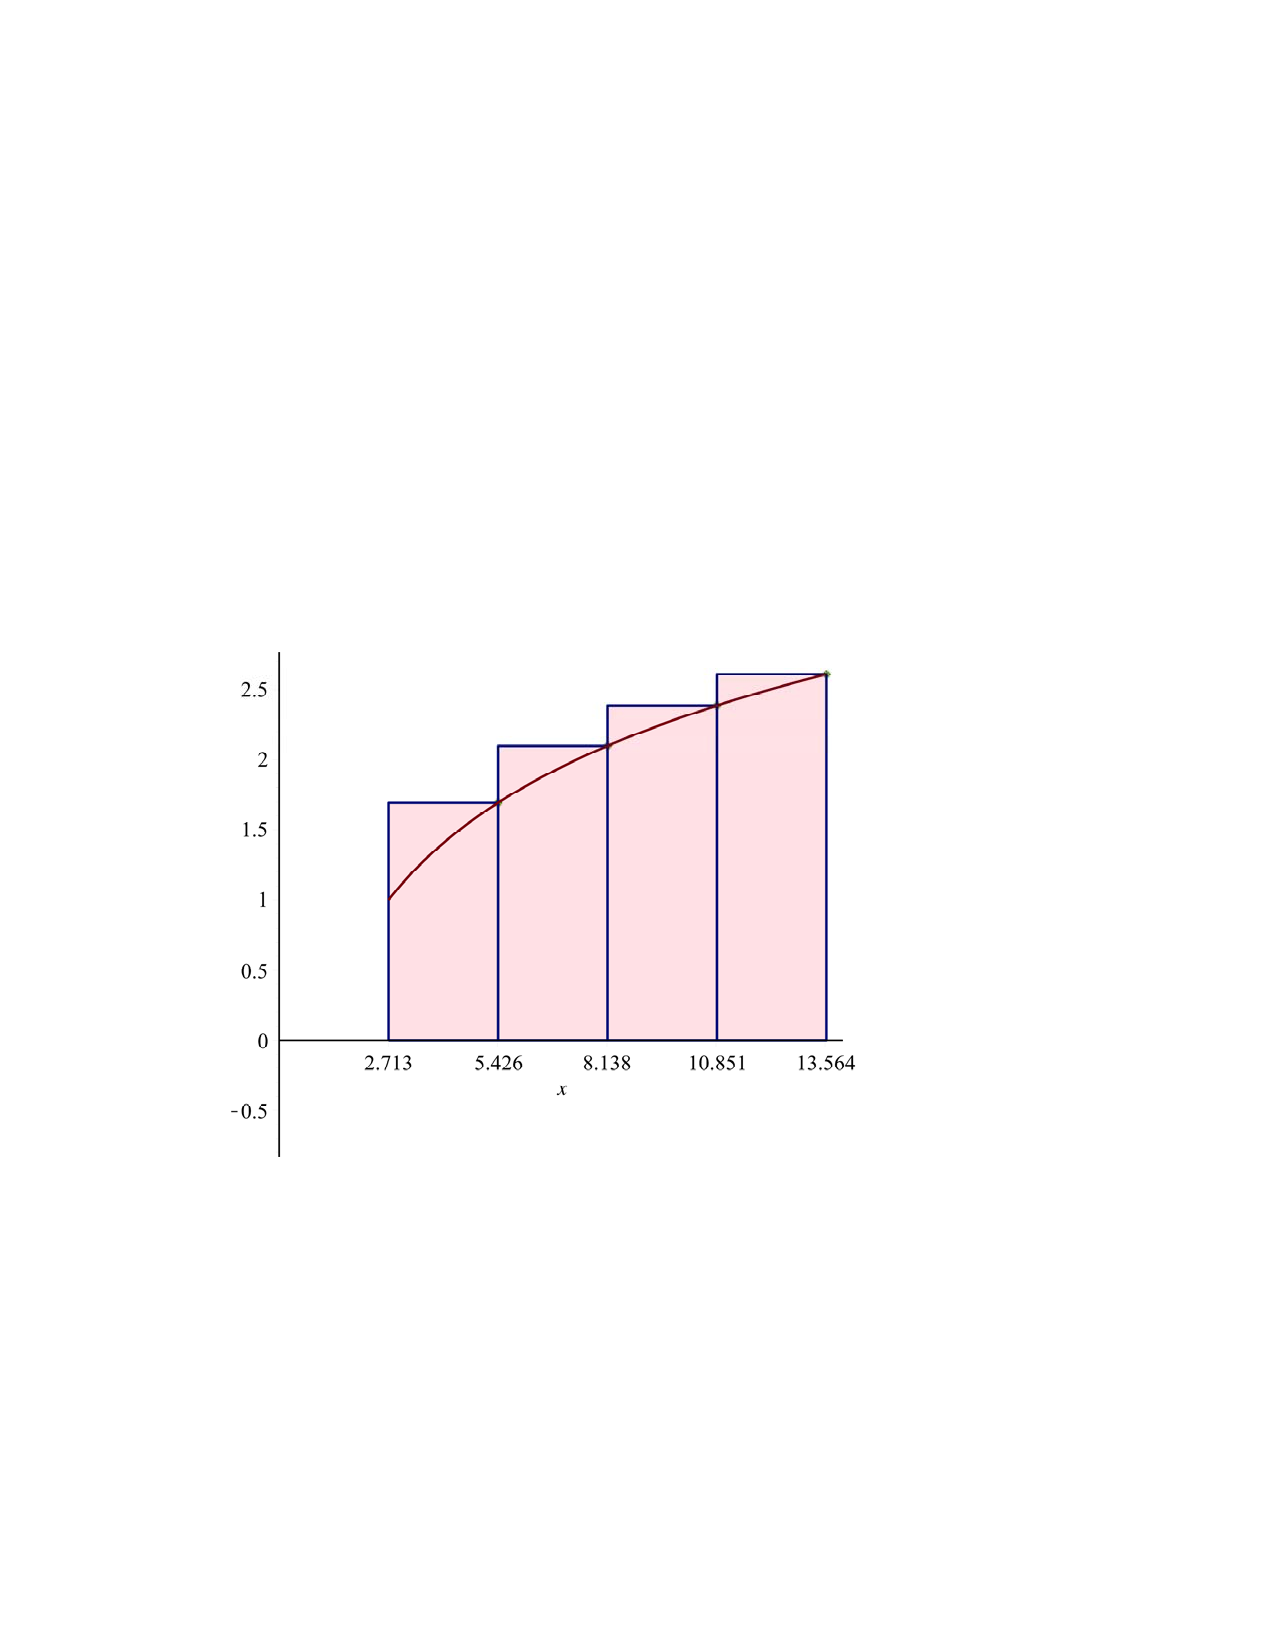
\includegraphics[scale=0.5]{log_right.pdf}\\
$A \approx e\ln{(2e)}+e\ln{(3e)}+e\ln{(4e)}+e\ln{(5e)}\approx 23.89$\\
This is an overestimate.}}} \fi

\item Sketch the graph of $f(x)$ on the interval $[e,5e]$.  Divide the interval into 4 subintervals of equal width.  On each subinterval, sketch a rectangle using the function value at the {\bf left endpoint} as the height of the rectangle on that subinterval.  Estimate the area between the graph of $f(x)$ and the $x$-axis on the interval $[e,5e]$ using the 4 rectangles that you sketched.  Is your estimate an overestimate or an underestimate?

\ifans{\fbox{\parbox{0.55\linewidth}{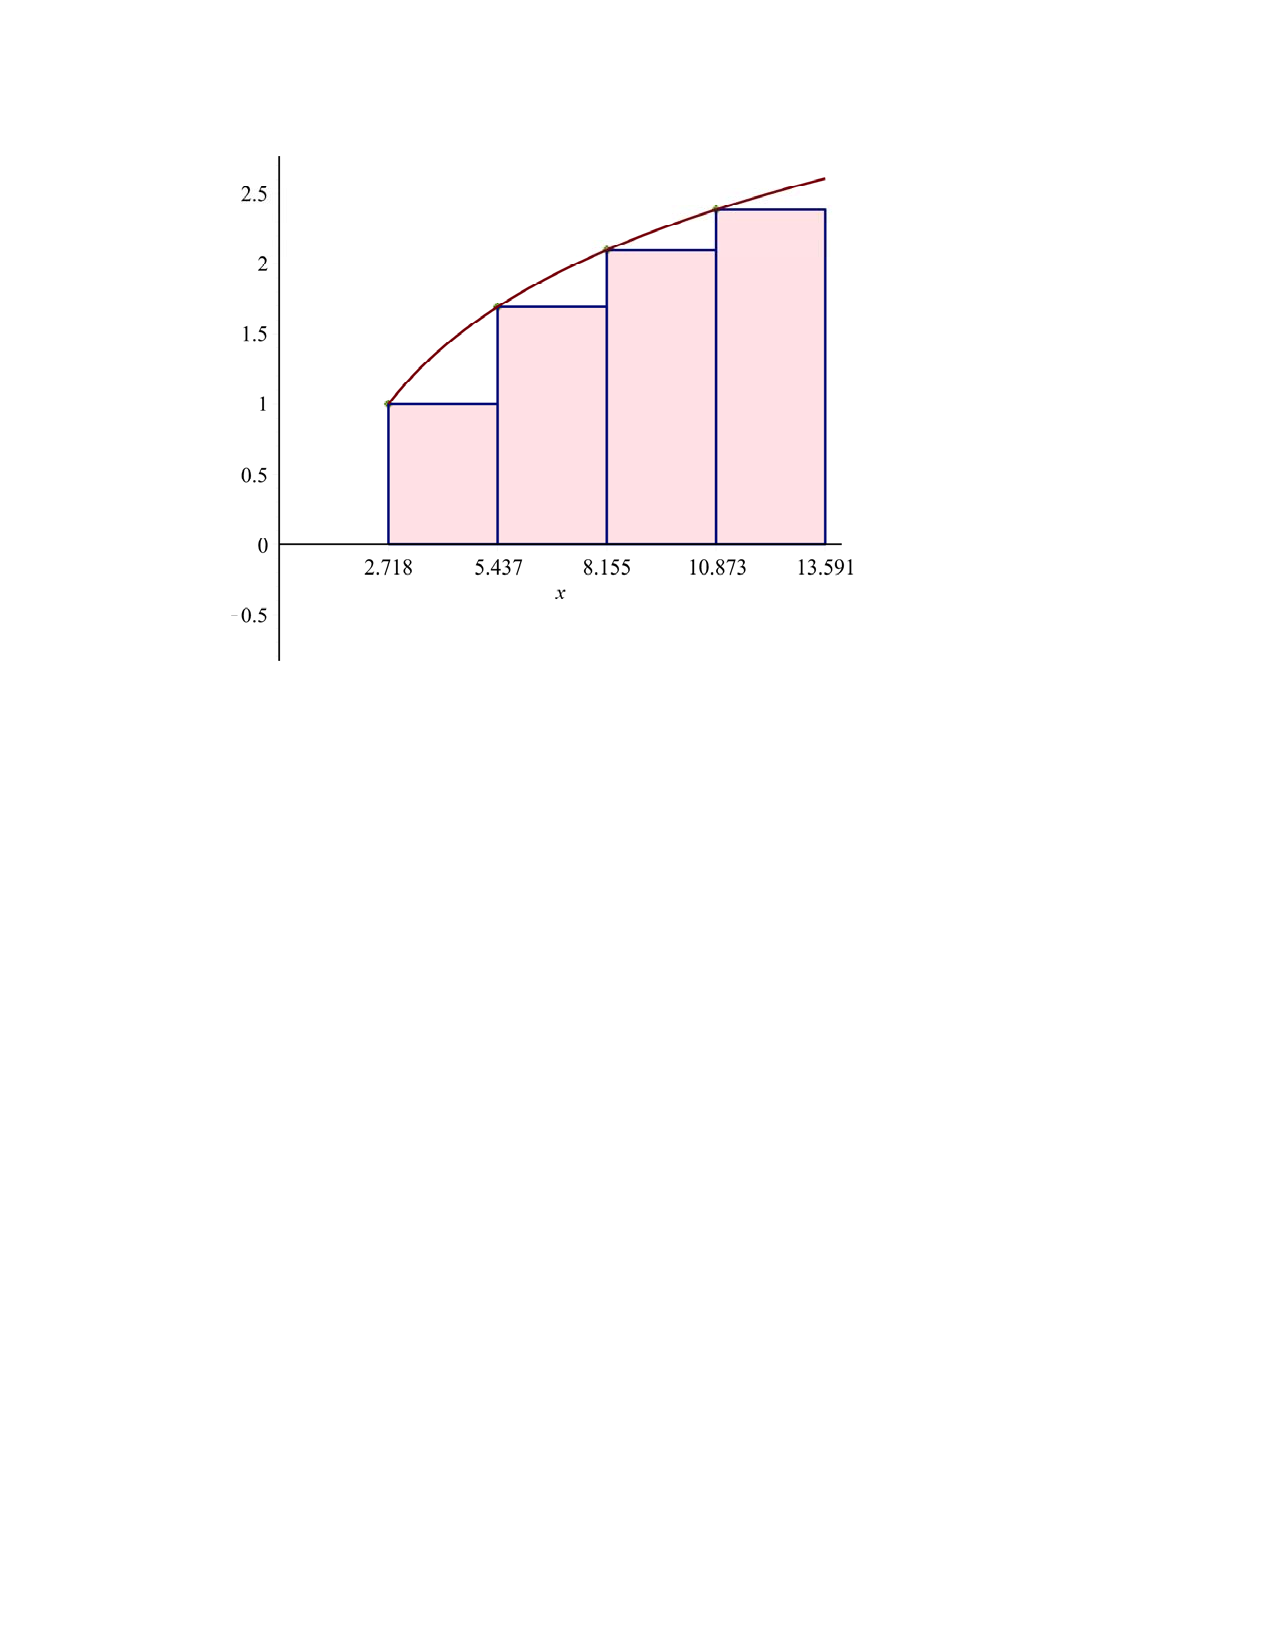
\includegraphics[scale=0.5]{log_left.pdf}\\
$A \approx e+e\ln{(2e)}+e\ln{(3e)}+e\ln{(4e)}\approx 19.51$\\
This is an underestimate.}}} \fi

\end{enumerate}

\item Let $f(x)=x^2+1$.  By the end of this problem, you will have computed the exact area under the graph of $f(x)$ on the interval $[1,6]$.

\begin{enumerate}

\item Find the $\Delta x$ which is necessary to divide $[1,6]$ into $n$ subintervals of equal width.

\ifans{\fbox{$\Delta x=\frac{5}{n}$}} \fi

\item In each of the $n$ subintervals of equal width, pick $x_k^*$ to be the right endpoint.  Fill in the following table:

\begin{center}
\begin{tabular}{c|c|c}
Subinterval Number & Right Endpoint Number & Right Endpoint of Subinterval\\
\hline
$k=1$ & $x_1^*$ & \ifans{\fbox{$1+\frac{5}{n}$}} \fi\\
\hline
$k=2$ & $x_2^*$ & \ifans{\fbox{$1+\frac{5}{n}(2)$}} \fi\\
\hline
$k=3$ & $x_3^*$ & \ifans{\fbox{$1+\frac{5}{n}(3)$}} \fi \\
\hline
. & . & .\\
. & . & .\\ 
. & . & .\\
\hline
$k=n-1$ & $x_{n-1}^*$ & \ifans{\fbox{$1+\frac{5}{n}(n-1)$}} \fi\\
\hline
$k=n$ & $x_{n}^*$ & \ifans{\fbox{$1+\frac{5}{n}(n)=6$}} \fi\\
\end{tabular}
\end{center}

\item {\bf Fill in the blank:} A closed formula for the right endpoints found in the table above is $x_k^*=\underline{\hspace{2 cm} \ifans{\fbox{$1+\frac{5}{n}(k)$}} \fi \hspace{2cm}}$, for $k=1,2,...,n-1,n$.

\item Determine $f(x_k^*)$, the height of the $k^{th}$ rectangle.

\ifans{\fbox{$\left(1+\frac{5}{n}k\right)^2+1$}} \fi

\item The right endpoint approximation of the area under the graph of $f(x)$ on the interval $[1,6]$ using $n$ rectangles of equal width is:\\

\begin{center}
$A \approx f(x_1^*)\Delta x+f(x_2^*)\Delta x+...+f(x_{n-1}^*)\Delta x+f(x_n^*)\Delta x=\sum_{k=1}^n{f(x_k^*)\Delta x}$
\end{center}

Using the appropriate formulas from the top of page 1, express the right endpoint approximation in closed form.

\ifans{\fbox{$\sum_{k=1}^n{f(x_k^*)\Delta x}=\sum_{k=1}^n\left[\left(1+\frac{5}{n}k\right)^2+1\right]\frac{5}{n}=10+\frac{25(n+1)}{n}+\frac{125(n+1)(2n+1)}{6n^2}$}} \fi

\item Repeating over finer and finer partitions is equivalent to the number of subintervals, $n$, approaching infinity.  Using this information, compute the exact area under the graph of $f(x)=x^2+1$ on the interval $[1,6]$.

\ifans{\fbox{$\frac{230}{3}$}}\fi

\end{enumerate}

\item For each of the following, use sigma notation and the appropriate summation formulas to evaluate the net signed area between the graph of $f(x)$ and the $x$-axis on the given interval.  Let $x_k^*$ be the {\bf right endpoint} of the $k^{th}$ subinterval (where all subintervals have equal width).

\begin{enumerate}

\item $f(x)=x-3$ on $[1,5]$

\ifans{\fbox{0}} \fi

\item $f(x)=\frac{x^2}{3}$ on $[2,5]$

\ifans{\fbox{13}} \fi

\item $f(x)=x^3-1$ on $[0,2]$

\ifans{\fbox{2}} \fi

\end{enumerate}

\item For each of the following, use sigma notation and the appropriate summation formulas to evaluate the net signed area between the graph of $f(x)$ and the $x$-axis on the given interval.  Let $x_k^*$ be the {\bf left endpoint} of the $k^{th}$ subinterval (where all subintervals have equal width).

\begin{enumerate}

\item $f(x)=x-3$ on $[1,5]$

\ifans{\fbox{0}} \fi

\item $f(x)=\frac{x^2}{3}$ on $[2,5]$

\ifans{\fbox{13}} \fi

\item $f(x)=x^3-1$ on $[0,2]$

\ifans{\fbox{2}} \fi

\end{enumerate}

\item For each of the following, use sigma notation and the appropriate summation formulas to evaluate the net signed area between the graph of $f(x)$ and the $x$-axis on the given interval.  Let $x_k^*$ be the {\bf midpoint} of the $k^{th}$ subinterval (where all subintervals have equal width).

\begin{enumerate}

\item $f(x)=x-3$ on $[1,5]$

\ifans{\fbox{0}} \fi

\item $f(x)=\frac{x^2}{3}$ on $[2,5]$

\ifans{\fbox{13}} \fi

\end{enumerate}

\item Use sigma notation and the appropriate summation formulas to formulate an expression which represents the net signed area between the graph of $f(x)=\cos{x}$ and the $x$-axis on the interval $[-\pi,\pi]$.  Let $x_k^*$ be the {\bf right endpoint} of the $k^{th}$ subinterval (where all subintervals have equal width).  DO NOT EVALUATE YOUR EXPRESSION.

\ifans{\fbox{$\sum_{k=1}^n\cos{\left(-\pi+\frac{2\pi}{n}k\right)}\frac{2\pi}{n}$}} \fi

\medskip

\item A \underline{Regular Polygon} is a polygon that is equiangular (all angles are equal in measure) and equilateral (all sides have the same length).  The diagram below shows several regular polygons inscribed within a circle of radius $r$.

\begin{center}

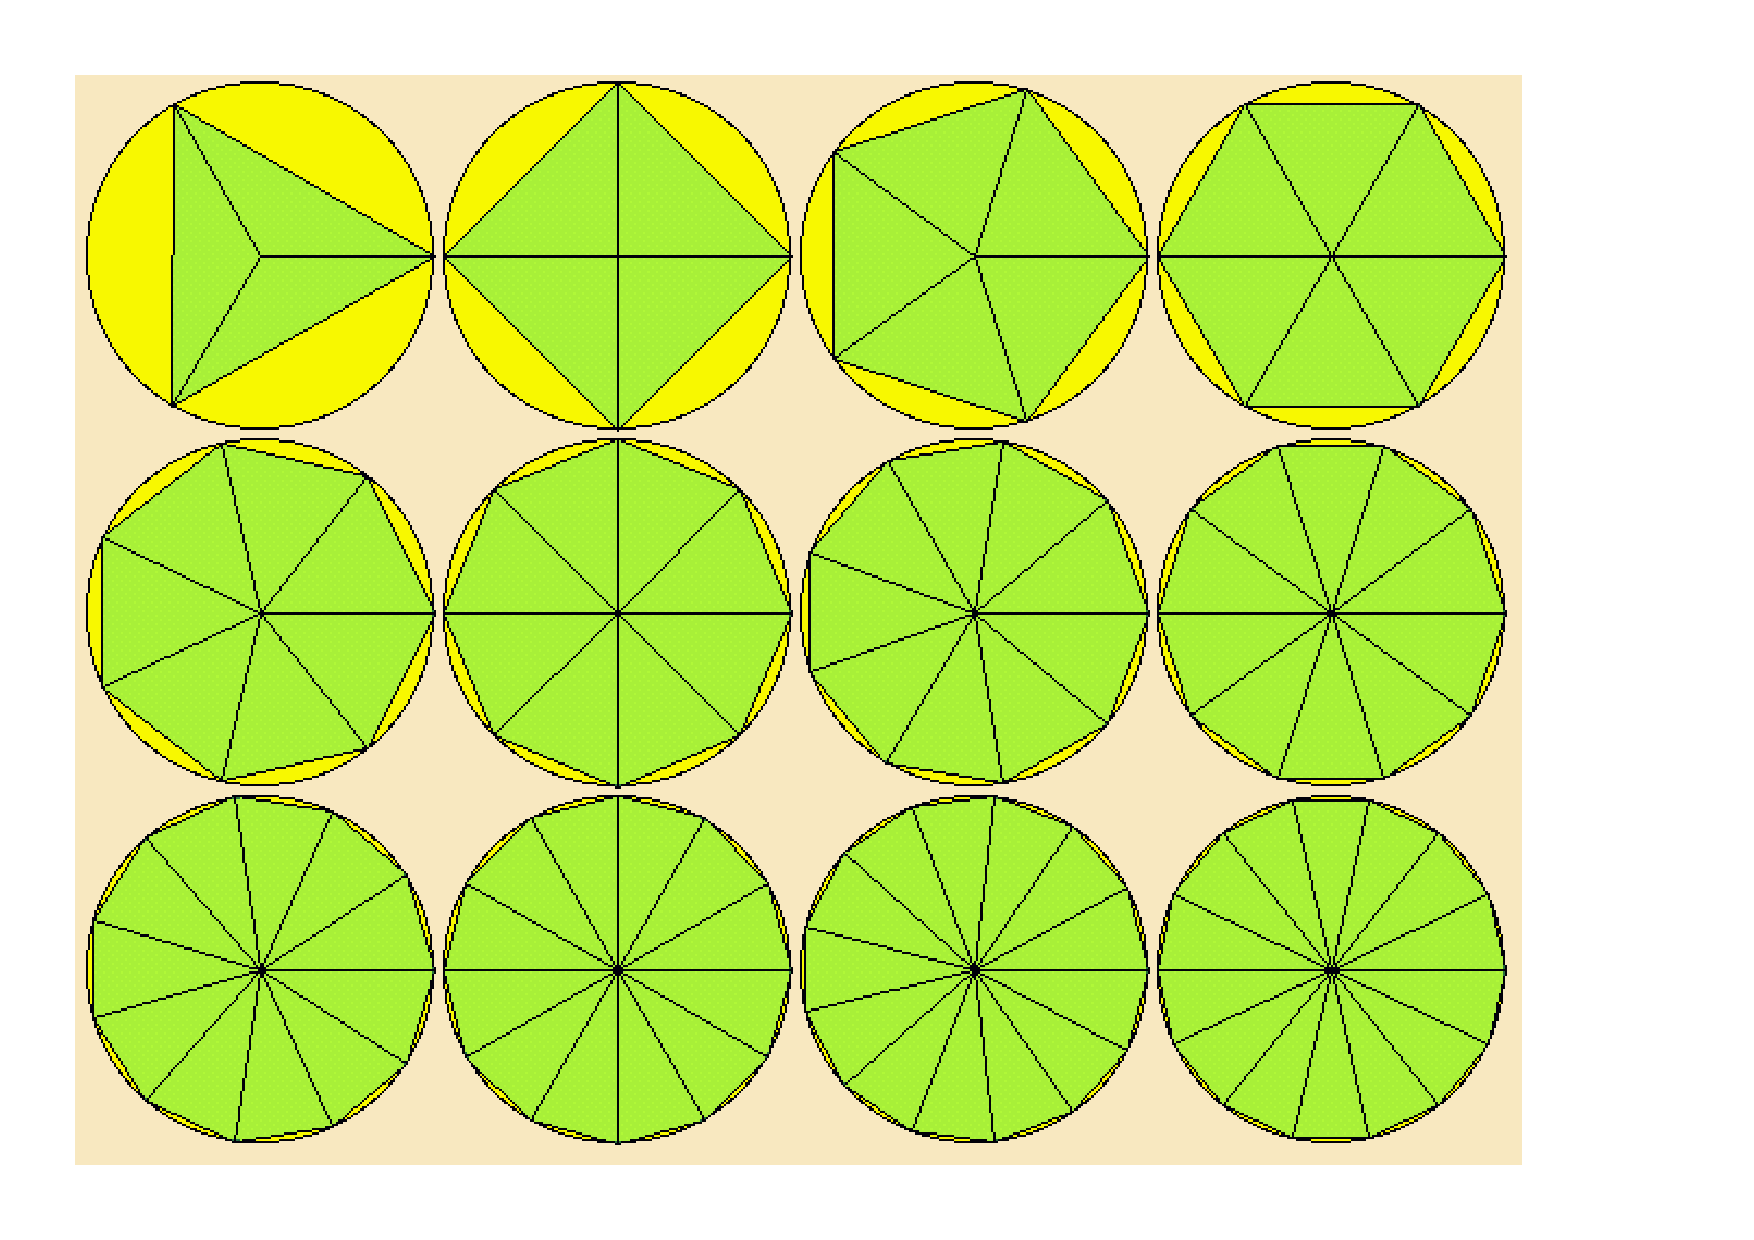
\includegraphics[scale=0.4]{Inscribed.pdf}

\end{center}

\begin{enumerate}

\item Let $A_n$ be the area of a regular $n$-sided polygon inscribed within a circle of radius $r$.  Divide the polygon into $n$ congruent triangles each with a central angle of $\frac{2\pi}{n}$ radians, as shown in the diagram above for several different values of $n$.    Show that $A_n=\frac{1}{2}r^2 \sin{\left(\frac{2\pi}{n}\right)} n$.

\ifans{\fbox{\parbox{1\linewidth}{We begin by examining one of the $n$ triangles, pictured below.
\begin{center}
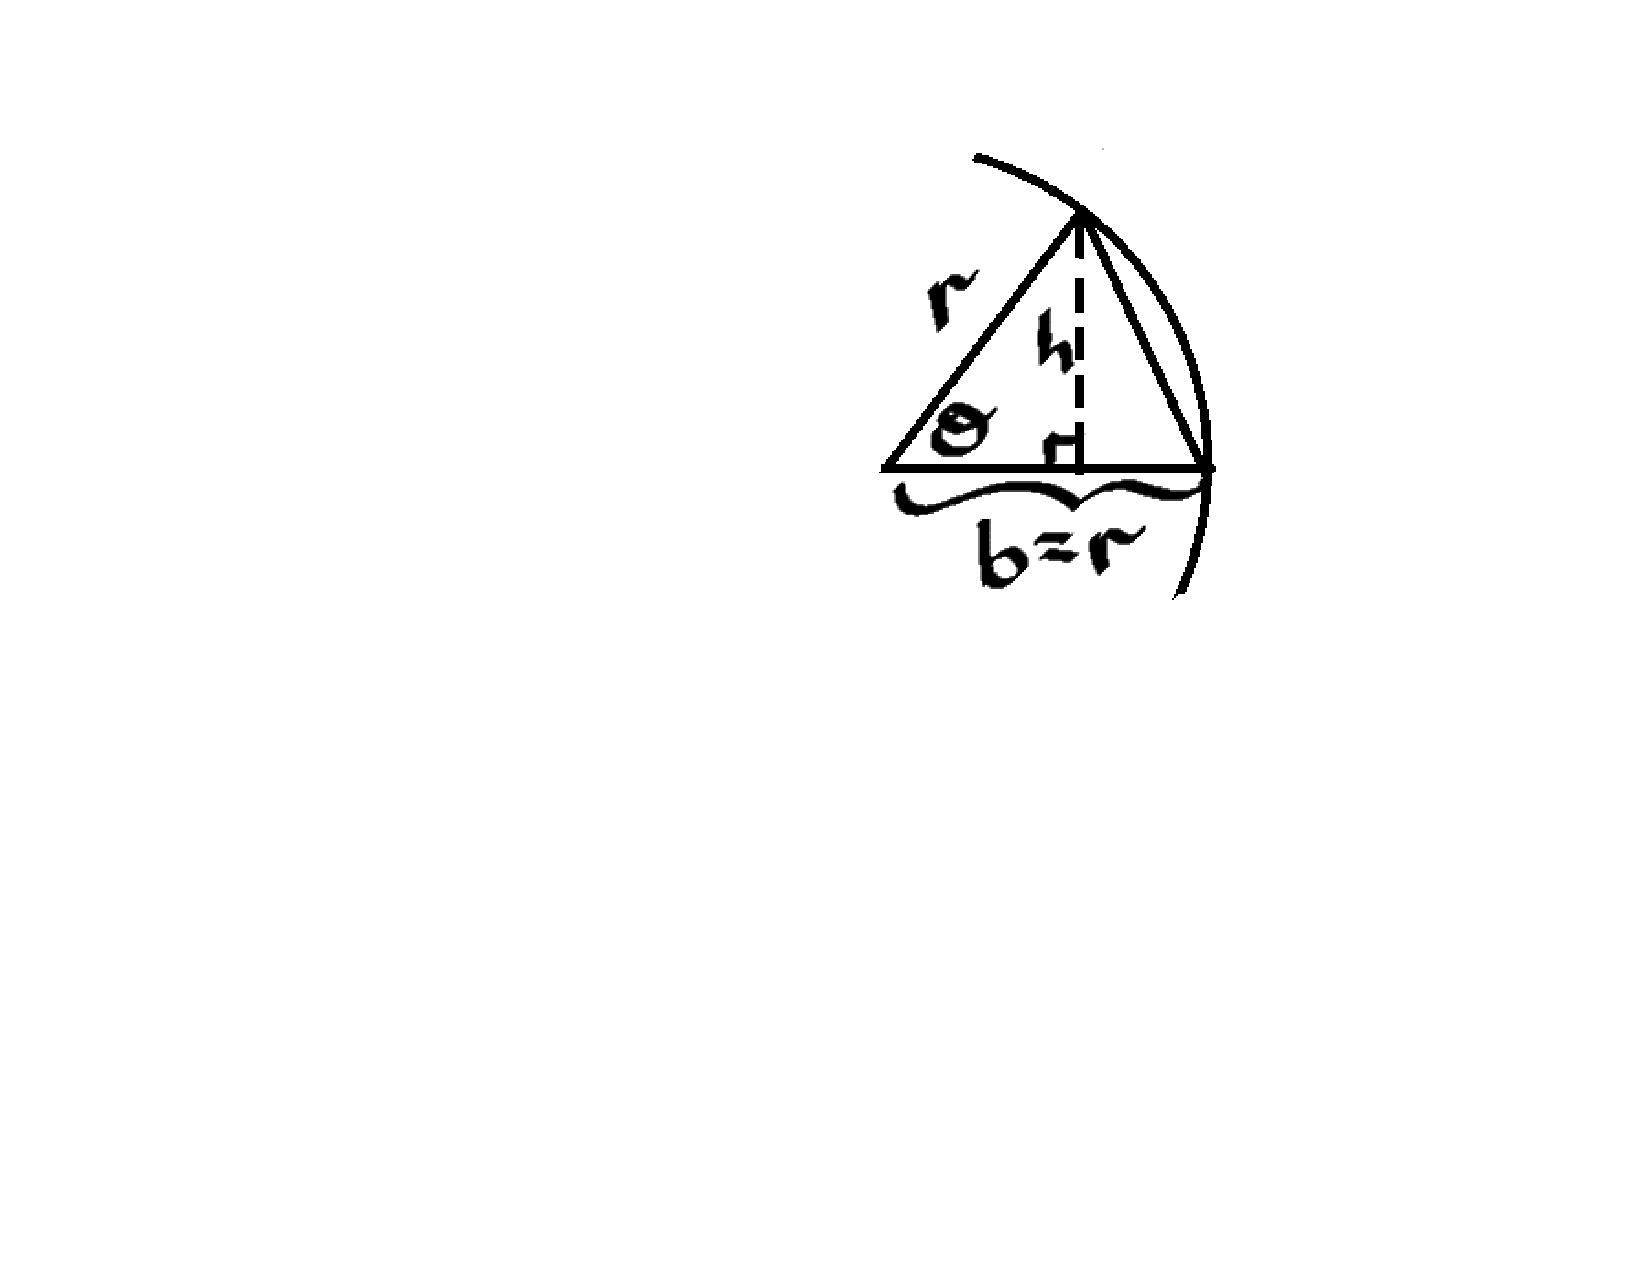
\includegraphics[scale=0.4]{triangle.pdf}
\end{center}
The base of the triangle has a length of $r$.  And, the height of the triangle is $r\sin{\theta}$, where $\theta$ is the central angle, $\frac{2\pi}{n}$.    Thus, the area of one triangle is:
$$A=\frac{1}{2}(r)\left(r\sin{\left(\frac{2\pi}{n}\right)}\right)=\frac{1}{2}r^2\sin{\left(\frac{2\pi}{n}\right)}$$
 But, the polygon is composed of $n$ such triangles.  So, the area of a regular $n$-sided polygon inscribed in the circle of radius $r$ is: 
$$A_n=\frac{1}{2}r^2\sin{\left(\frac{2\pi}{n}\right)}n$$
}}} \fi

\item What can you conclude about the area of the $n$-sided polygon as the number of sides of the polygon, $n$, approaches infinity?  In other words, compute $\lim_{n \rightarrow \infty}{A_n}$.

\ifans{\fbox{$\lim_{n \rightarrow \infty}{A_n}=\pi r^2$}} \fi

\end{enumerate}

\end{enumerate}

\end{document}